% Created by tikzDevice version 0.10.1 on 2017-05-28 17:05:20
% !TEX encoding = UTF-8 Unicode
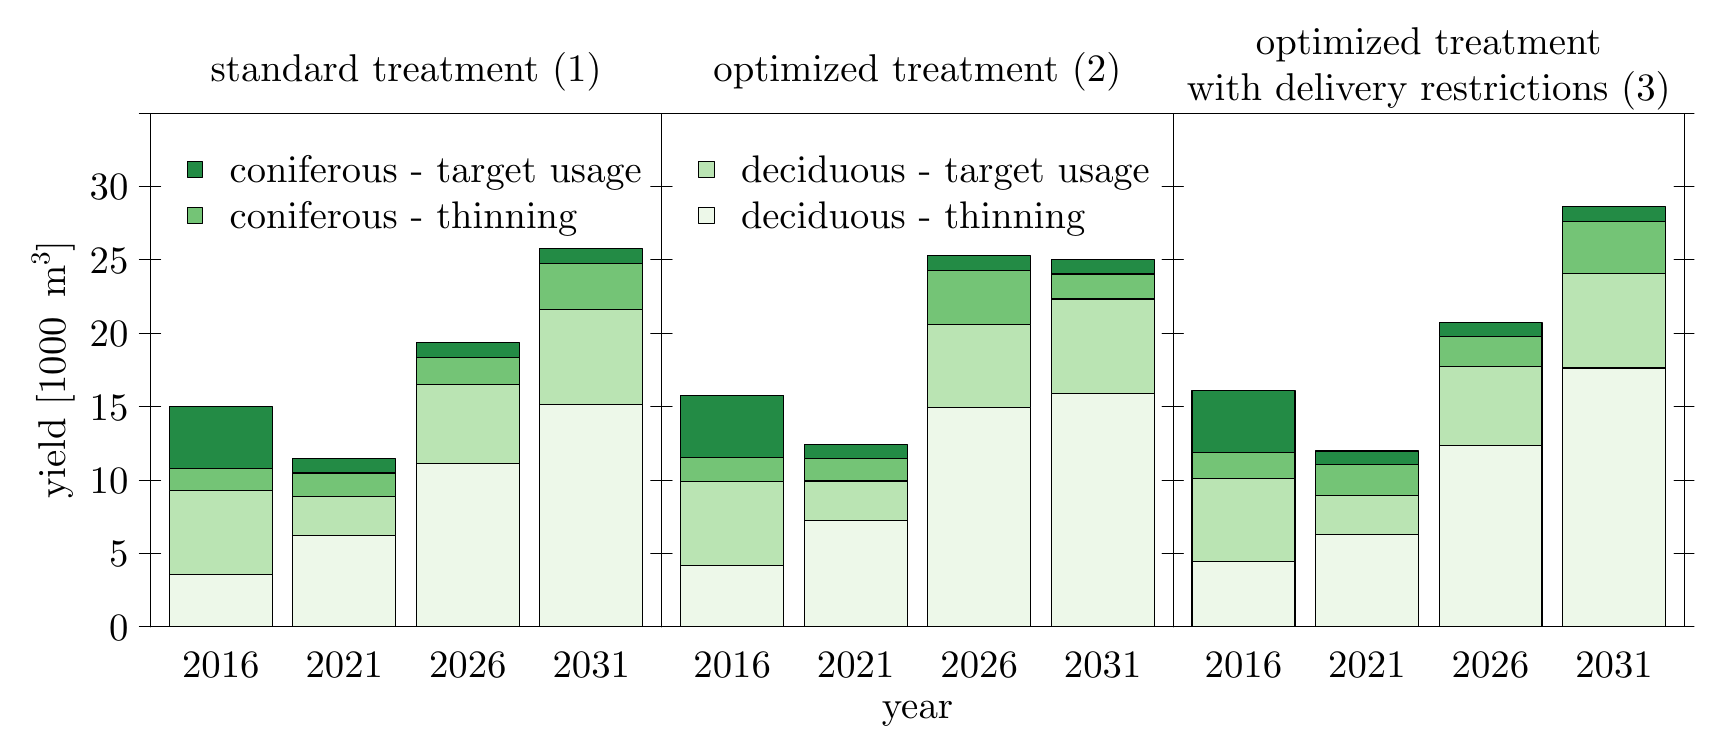
\begin{tikzpicture}[x=1pt,y=1pt]
\definecolor{fillColor}{RGB}{255,255,255}
\path[use as bounding box,fill=fillColor,fill opacity=0.00] (0,0) rectangle (602.23,252.94);
\begin{scope}
\path[clip] ( 44.35, 36.43) rectangle (229.12,222.06);
\definecolor{drawColor}{RGB}{0,0,0}
\definecolor{fillColor}{RGB}{237,248,233}

\path[draw=drawColor,line width= 0.4pt,line join=round,line cap=round,fill=fillColor] ( 51.20, 36.43) rectangle ( 88.39, 55.44);
\definecolor{fillColor}{RGB}{186,228,179}

\path[draw=drawColor,line width= 0.4pt,line join=round,line cap=round,fill=fillColor] ( 51.20, 55.44) rectangle ( 88.39, 85.61);
\definecolor{fillColor}{RGB}{116,196,118}

\path[draw=drawColor,line width= 0.4pt,line join=round,line cap=round,fill=fillColor] ( 51.20, 85.61) rectangle ( 88.39, 93.58);
\definecolor{fillColor}{RGB}{35,139,69}

\path[draw=drawColor,line width= 0.4pt,line join=round,line cap=round,fill=fillColor] ( 51.20, 93.58) rectangle ( 88.39,115.99);
\definecolor{fillColor}{RGB}{237,248,233}

\path[draw=drawColor,line width= 0.4pt,line join=round,line cap=round,fill=fillColor] ( 95.83, 36.43) rectangle (133.02, 69.30);
\definecolor{fillColor}{RGB}{186,228,179}

\path[draw=drawColor,line width= 0.4pt,line join=round,line cap=round,fill=fillColor] ( 95.83, 69.30) rectangle (133.02, 83.47);
\definecolor{fillColor}{RGB}{116,196,118}

\path[draw=drawColor,line width= 0.4pt,line join=round,line cap=round,fill=fillColor] ( 95.83, 83.47) rectangle (133.02, 92.03);
\definecolor{fillColor}{RGB}{35,139,69}

\path[draw=drawColor,line width= 0.4pt,line join=round,line cap=round,fill=fillColor] ( 95.83, 92.03) rectangle (133.02, 97.23);
\definecolor{fillColor}{RGB}{237,248,233}

\path[draw=drawColor,line width= 0.4pt,line join=round,line cap=round,fill=fillColor] (140.46, 36.43) rectangle (177.65, 95.54);
\definecolor{fillColor}{RGB}{186,228,179}

\path[draw=drawColor,line width= 0.4pt,line join=round,line cap=round,fill=fillColor] (140.46, 95.54) rectangle (177.65,124.12);
\definecolor{fillColor}{RGB}{116,196,118}

\path[draw=drawColor,line width= 0.4pt,line join=round,line cap=round,fill=fillColor] (140.46,124.12) rectangle (177.65,133.86);
\definecolor{fillColor}{RGB}{35,139,69}

\path[draw=drawColor,line width= 0.4pt,line join=round,line cap=round,fill=fillColor] (140.46,133.86) rectangle (177.65,139.05);
\definecolor{fillColor}{RGB}{237,248,233}

\path[draw=drawColor,line width= 0.4pt,line join=round,line cap=round,fill=fillColor] (185.09, 36.43) rectangle (222.28,116.81);
\definecolor{fillColor}{RGB}{186,228,179}

\path[draw=drawColor,line width= 0.4pt,line join=round,line cap=round,fill=fillColor] (185.09,116.81) rectangle (222.28,151.00);
\definecolor{fillColor}{RGB}{116,196,118}

\path[draw=drawColor,line width= 0.4pt,line join=round,line cap=round,fill=fillColor] (185.09,151.00) rectangle (222.28,167.82);
\definecolor{fillColor}{RGB}{35,139,69}

\path[draw=drawColor,line width= 0.4pt,line join=round,line cap=round,fill=fillColor] (185.09,167.82) rectangle (222.28,173.12);
\end{scope}
\begin{scope}
\path[clip] (  0.00,  0.00) rectangle (602.23,252.94);
\definecolor{drawColor}{RGB}{0,0,0}

\node[text=drawColor,anchor=base,inner sep=0pt, outer sep=0pt, scale=  1.40] at (136.74,233.66) {standard treatment (1)};

\path[draw=drawColor,line width= 0.4pt,line join=round,line cap=round] ( 44.35, 36.43) -- ( 40.39, 36.43);

\path[draw=drawColor,line width= 0.4pt,line join=round,line cap=round] ( 44.35, 62.95) -- ( 40.39, 62.95);

\path[draw=drawColor,line width= 0.4pt,line join=round,line cap=round] ( 44.35, 89.47) -- ( 40.39, 89.47);

\path[draw=drawColor,line width= 0.4pt,line join=round,line cap=round] ( 44.35,115.99) -- ( 40.39,115.99);

\path[draw=drawColor,line width= 0.4pt,line join=round,line cap=round] ( 44.35,142.50) -- ( 40.39,142.50);

\path[draw=drawColor,line width= 0.4pt,line join=round,line cap=round] ( 44.35,169.02) -- ( 40.39,169.02);

\path[draw=drawColor,line width= 0.4pt,line join=round,line cap=round] ( 44.35,195.54) -- ( 40.39,195.54);

\path[draw=drawColor,line width= 0.4pt,line join=round,line cap=round] ( 44.35,222.06) -- ( 40.39,222.06);

\node[text=drawColor,anchor=base east,inner sep=0pt, outer sep=0pt, scale=  1.40] at ( 36.43, 31.61) {0};

\node[text=drawColor,anchor=base east,inner sep=0pt, outer sep=0pt, scale=  1.40] at ( 36.43, 58.13) {5};

\node[text=drawColor,anchor=base east,inner sep=0pt, outer sep=0pt, scale=  1.40] at ( 36.43, 84.65) {10};

\node[text=drawColor,anchor=base east,inner sep=0pt, outer sep=0pt, scale=  1.40] at ( 36.43,111.16) {15};

\node[text=drawColor,anchor=base east,inner sep=0pt, outer sep=0pt, scale=  1.40] at ( 36.43,137.68) {20};

\node[text=drawColor,anchor=base east,inner sep=0pt, outer sep=0pt, scale=  1.40] at ( 36.43,164.20) {25};

\node[text=drawColor,anchor=base east,inner sep=0pt, outer sep=0pt, scale=  1.40] at ( 36.43,190.72) {30};

\path[draw=drawColor,line width= 0.4pt,line join=round,line cap=round] ( 44.35, 36.43) -- ( 48.05, 36.43);

\path[draw=drawColor,line width= 0.4pt,line join=round,line cap=round] ( 44.35, 62.95) -- ( 48.05, 62.95);

\path[draw=drawColor,line width= 0.4pt,line join=round,line cap=round] ( 44.35, 89.47) -- ( 48.05, 89.47);

\path[draw=drawColor,line width= 0.4pt,line join=round,line cap=round] ( 44.35,115.99) -- ( 48.05,115.99);

\path[draw=drawColor,line width= 0.4pt,line join=round,line cap=round] ( 44.35,142.50) -- ( 48.05,142.50);

\path[draw=drawColor,line width= 0.4pt,line join=round,line cap=round] ( 44.35,169.02) -- ( 48.05,169.02);

\path[draw=drawColor,line width= 0.4pt,line join=round,line cap=round] ( 44.35,195.54) -- ( 48.05,195.54);

\node[text=drawColor,anchor=base,inner sep=0pt, outer sep=0pt, scale=  1.40] at ( 69.79, 18.22) {2016};

\node[text=drawColor,anchor=base,inner sep=0pt, outer sep=0pt, scale=  1.40] at (114.42, 18.22) {2021};

\node[text=drawColor,anchor=base,inner sep=0pt, outer sep=0pt, scale=  1.40] at (159.05, 18.22) {2026};

\node[text=drawColor,anchor=base,inner sep=0pt, outer sep=0pt, scale=  1.40] at (203.68, 18.22) {2031};

\node[text=drawColor,rotate= 90.00,anchor=base west,inner sep=0pt, outer sep=0pt, scale=  1.40] at ( 13.53, 82.67) {yield [1000};

\node[text=drawColor,rotate= 90.00,anchor=base west,inner sep=0pt, outer sep=0pt, scale=  1.40] at ( 13.53,148.37) { };

\node[text=drawColor,rotate= 90.00,anchor=base west,inner sep=0pt, outer sep=0pt, scale=  1.40] at ( 13.53,155.37) {m};

\node[text=drawColor,rotate= 90.00,anchor=base west,inner sep=0pt, outer sep=0pt, scale=  0.98] at (  7.80,167.04) {3};

\node[text=drawColor,rotate= 90.00,anchor=base west,inner sep=0pt, outer sep=0pt, scale=  1.40] at ( 13.53,171.93) {]};
\end{scope}
\begin{scope}
\path[clip] ( 44.35, 36.43) rectangle (229.12,222.06);
\definecolor{drawColor}{RGB}{0,0,0}
\definecolor{fillColor}{RGB}{35,139,69}

\path[draw=drawColor,line width= 0.4pt,line join=round,line cap=round,fill=fillColor] ( 57.76,198.95) rectangle ( 63.29,204.48);
\definecolor{fillColor}{RGB}{116,196,118}

\path[draw=drawColor,line width= 0.4pt,line join=round,line cap=round,fill=fillColor] ( 57.76,182.32) rectangle ( 63.29,187.84);

\node[text=drawColor,anchor=base west,inner sep=0pt, outer sep=0pt, scale=  1.39] at ( 73.00,196.94) {coniferous - target usage};

\node[text=drawColor,anchor=base west,inner sep=0pt, outer sep=0pt, scale=  1.39] at ( 73.00,180.31) {coniferous - thinning};
\end{scope}
\begin{scope}
\path[clip] (  0.00,  0.00) rectangle (602.23,252.94);
\definecolor{drawColor}{RGB}{0,0,0}

\path[draw=drawColor,line width= 0.4pt,line join=round,line cap=round] ( 44.35, 36.43) --
	(229.12, 36.43) --
	(229.12,222.06) --
	( 44.35,222.06) --
	( 44.35, 36.43);
\end{scope}
\begin{scope}
\path[clip] (229.12, 36.43) rectangle (413.89,222.06);
\definecolor{drawColor}{RGB}{0,0,0}
\definecolor{fillColor}{RGB}{237,248,233}

\path[draw=drawColor,line width= 0.4pt,line join=round,line cap=round,fill=fillColor] (235.97, 36.43) rectangle (273.16, 58.65);
\definecolor{fillColor}{RGB}{186,228,179}

\path[draw=drawColor,line width= 0.4pt,line join=round,line cap=round,fill=fillColor] (235.97, 58.65) rectangle (273.16, 88.82);
\definecolor{fillColor}{RGB}{116,196,118}

\path[draw=drawColor,line width= 0.4pt,line join=round,line cap=round,fill=fillColor] (235.97, 88.82) rectangle (273.16, 97.78);
\definecolor{fillColor}{RGB}{35,139,69}

\path[draw=drawColor,line width= 0.4pt,line join=round,line cap=round,fill=fillColor] (235.97, 97.78) rectangle (273.16,120.18);
\definecolor{fillColor}{RGB}{237,248,233}

\path[draw=drawColor,line width= 0.4pt,line join=round,line cap=round,fill=fillColor] (280.60, 36.43) rectangle (317.79, 74.94);
\definecolor{fillColor}{RGB}{186,228,179}

\path[draw=drawColor,line width= 0.4pt,line join=round,line cap=round,fill=fillColor] (280.60, 74.94) rectangle (317.79, 89.11);
\definecolor{fillColor}{RGB}{116,196,118}

\path[draw=drawColor,line width= 0.4pt,line join=round,line cap=round,fill=fillColor] (280.60, 89.11) rectangle (317.79, 97.11);
\definecolor{fillColor}{RGB}{35,139,69}

\path[draw=drawColor,line width= 0.4pt,line join=round,line cap=round,fill=fillColor] (280.60, 97.11) rectangle (317.79,102.31);
\definecolor{fillColor}{RGB}{237,248,233}

\path[draw=drawColor,line width= 0.4pt,line join=round,line cap=round,fill=fillColor] (325.23, 36.43) rectangle (362.42,115.65);
\definecolor{fillColor}{RGB}{186,228,179}

\path[draw=drawColor,line width= 0.4pt,line join=round,line cap=round,fill=fillColor] (325.23,115.65) rectangle (362.42,145.67);
\definecolor{fillColor}{RGB}{116,196,118}

\path[draw=drawColor,line width= 0.4pt,line join=round,line cap=round,fill=fillColor] (325.23,145.67) rectangle (362.42,165.29);
\definecolor{fillColor}{RGB}{35,139,69}

\path[draw=drawColor,line width= 0.4pt,line join=round,line cap=round,fill=fillColor] (325.23,165.29) rectangle (362.42,170.48);
\definecolor{fillColor}{RGB}{237,248,233}

\path[draw=drawColor,line width= 0.4pt,line join=round,line cap=round,fill=fillColor] (369.86, 36.43) rectangle (407.05,120.67);
\definecolor{fillColor}{RGB}{186,228,179}

\path[draw=drawColor,line width= 0.4pt,line join=round,line cap=round,fill=fillColor] (369.86,120.67) rectangle (407.05,154.91);
\definecolor{fillColor}{RGB}{116,196,118}

\path[draw=drawColor,line width= 0.4pt,line join=round,line cap=round,fill=fillColor] (369.86,154.91) rectangle (407.05,163.93);
\definecolor{fillColor}{RGB}{35,139,69}

\path[draw=drawColor,line width= 0.4pt,line join=round,line cap=round,fill=fillColor] (369.86,163.93) rectangle (407.05,169.22);
\end{scope}
\begin{scope}
\path[clip] (  0.00,  0.00) rectangle (602.23,252.94);
\definecolor{drawColor}{RGB}{0,0,0}

\path[draw=drawColor,line width= 0.4pt,line join=round,line cap=round] (229.12, 36.43) -- (225.16, 36.43);

\path[draw=drawColor,line width= 0.4pt,line join=round,line cap=round] (229.12, 62.95) -- (225.16, 62.95);

\path[draw=drawColor,line width= 0.4pt,line join=round,line cap=round] (229.12, 89.47) -- (225.16, 89.47);

\path[draw=drawColor,line width= 0.4pt,line join=round,line cap=round] (229.12,115.99) -- (225.16,115.99);

\path[draw=drawColor,line width= 0.4pt,line join=round,line cap=round] (229.12,142.50) -- (225.16,142.50);

\path[draw=drawColor,line width= 0.4pt,line join=round,line cap=round] (229.12,169.02) -- (225.16,169.02);

\path[draw=drawColor,line width= 0.4pt,line join=round,line cap=round] (229.12,195.54) -- (225.16,195.54);

\path[draw=drawColor,line width= 0.4pt,line join=round,line cap=round] (229.12, 36.43) -- (232.82, 36.43);

\path[draw=drawColor,line width= 0.4pt,line join=round,line cap=round] (229.12, 62.95) -- (232.82, 62.95);

\path[draw=drawColor,line width= 0.4pt,line join=round,line cap=round] (229.12, 89.47) -- (232.82, 89.47);

\path[draw=drawColor,line width= 0.4pt,line join=round,line cap=round] (229.12,115.99) -- (232.82,115.99);

\path[draw=drawColor,line width= 0.4pt,line join=round,line cap=round] (229.12,142.50) -- (232.82,142.50);

\path[draw=drawColor,line width= 0.4pt,line join=round,line cap=round] (229.12,169.02) -- (232.82,169.02);

\path[draw=drawColor,line width= 0.4pt,line join=round,line cap=round] (229.12,195.54) -- (232.82,195.54);

\node[text=drawColor,anchor=base,inner sep=0pt, outer sep=0pt, scale=  1.40] at (254.56, 18.22) {2016};

\node[text=drawColor,anchor=base,inner sep=0pt, outer sep=0pt, scale=  1.40] at (299.19, 18.22) {2021};

\node[text=drawColor,anchor=base,inner sep=0pt, outer sep=0pt, scale=  1.40] at (343.82, 18.22) {2026};

\node[text=drawColor,anchor=base,inner sep=0pt, outer sep=0pt, scale=  1.40] at (388.45, 18.22) {2031};

\path[draw=drawColor,line width= 0.4pt,line join=round,line cap=round] (229.12, 36.43) --
	(413.89, 36.43) --
	(413.89,222.06) --
	(229.12,222.06) --
	(229.12, 36.43);
\end{scope}
\begin{scope}
\path[clip] (229.12, 36.43) rectangle (413.89,222.06);
\definecolor{drawColor}{RGB}{0,0,0}
\definecolor{fillColor}{RGB}{186,228,179}

\path[draw=drawColor,line width= 0.4pt,line join=round,line cap=round,fill=fillColor] (242.53,198.95) rectangle (248.06,204.48);
\definecolor{fillColor}{RGB}{237,248,233}

\path[draw=drawColor,line width= 0.4pt,line join=round,line cap=round,fill=fillColor] (242.53,182.32) rectangle (248.06,187.84);

\node[text=drawColor,anchor=base west,inner sep=0pt, outer sep=0pt, scale=  1.39] at (257.77,196.94) {deciduous - target usage};

\node[text=drawColor,anchor=base west,inner sep=0pt, outer sep=0pt, scale=  1.39] at (257.77,180.31) {deciduous - thinning};
\end{scope}
\begin{scope}
\path[clip] (  0.00,  0.00) rectangle (602.23,252.94);
\definecolor{drawColor}{RGB}{0,0,0}

\node[text=drawColor,anchor=base,inner sep=0pt, outer sep=0pt, scale=  1.40] at (321.51,233.66) {optimized treatment (2)};

\node[text=drawColor,anchor=base,inner sep=0pt, outer sep=0pt, scale=  1.40] at (321.51,  3.17) {year};
\end{scope}
\begin{scope}
\path[clip] (413.89, 36.43) rectangle (598.66,222.06);
\definecolor{drawColor}{RGB}{0,0,0}
\definecolor{fillColor}{RGB}{237,248,233}

\path[draw=drawColor,line width= 0.4pt,line join=round,line cap=round,fill=fillColor] (420.74, 36.43) rectangle (457.93, 59.98);
\definecolor{fillColor}{RGB}{186,228,179}

\path[draw=drawColor,line width= 0.4pt,line join=round,line cap=round,fill=fillColor] (420.74, 59.98) rectangle (457.93, 90.15);
\definecolor{fillColor}{RGB}{116,196,118}

\path[draw=drawColor,line width= 0.4pt,line join=round,line cap=round,fill=fillColor] (420.74, 90.15) rectangle (457.93, 99.50);
\definecolor{fillColor}{RGB}{35,139,69}

\path[draw=drawColor,line width= 0.4pt,line join=round,line cap=round,fill=fillColor] (420.74, 99.50) rectangle (457.93,121.90);
\definecolor{fillColor}{RGB}{237,248,233}

\path[draw=drawColor,line width= 0.4pt,line join=round,line cap=round,fill=fillColor] (465.37, 36.43) rectangle (502.56, 69.78);
\definecolor{fillColor}{RGB}{186,228,179}

\path[draw=drawColor,line width= 0.4pt,line join=round,line cap=round,fill=fillColor] (465.37, 69.78) rectangle (502.56, 83.95);
\definecolor{fillColor}{RGB}{116,196,118}

\path[draw=drawColor,line width= 0.4pt,line join=round,line cap=round,fill=fillColor] (465.37, 83.95) rectangle (502.56, 95.14);
\definecolor{fillColor}{RGB}{35,139,69}

\path[draw=drawColor,line width= 0.4pt,line join=round,line cap=round,fill=fillColor] (465.37, 95.14) rectangle (502.56, 99.98);
\definecolor{fillColor}{RGB}{237,248,233}

\path[draw=drawColor,line width= 0.4pt,line join=round,line cap=round,fill=fillColor] (510.00, 36.43) rectangle (547.19,102.08);
\definecolor{fillColor}{RGB}{186,228,179}

\path[draw=drawColor,line width= 0.4pt,line join=round,line cap=round,fill=fillColor] (510.00,102.08) rectangle (547.19,130.66);
\definecolor{fillColor}{RGB}{116,196,118}

\path[draw=drawColor,line width= 0.4pt,line join=round,line cap=round,fill=fillColor] (510.00,130.66) rectangle (547.19,141.26);
\definecolor{fillColor}{RGB}{35,139,69}

\path[draw=drawColor,line width= 0.4pt,line join=round,line cap=round,fill=fillColor] (510.00,141.26) rectangle (547.19,146.46);
\definecolor{fillColor}{RGB}{237,248,233}

\path[draw=drawColor,line width= 0.4pt,line join=round,line cap=round,fill=fillColor] (554.63, 36.43) rectangle (591.82,129.95);
\definecolor{fillColor}{RGB}{186,228,179}

\path[draw=drawColor,line width= 0.4pt,line join=round,line cap=round,fill=fillColor] (554.63,129.95) rectangle (591.82,164.16);
\definecolor{fillColor}{RGB}{116,196,118}

\path[draw=drawColor,line width= 0.4pt,line join=round,line cap=round,fill=fillColor] (554.63,164.16) rectangle (591.82,182.92);
\definecolor{fillColor}{RGB}{35,139,69}

\path[draw=drawColor,line width= 0.4pt,line join=round,line cap=round,fill=fillColor] (554.63,182.92) rectangle (591.82,188.21);
\end{scope}
\begin{scope}
\path[clip] (  0.00,  0.00) rectangle (602.23,252.94);
\definecolor{drawColor}{RGB}{0,0,0}

\path[draw=drawColor,line width= 0.4pt,line join=round,line cap=round] (413.89, 36.43) -- (409.93, 36.43);

\path[draw=drawColor,line width= 0.4pt,line join=round,line cap=round] (413.89, 62.95) -- (409.93, 62.95);

\path[draw=drawColor,line width= 0.4pt,line join=round,line cap=round] (413.89, 89.47) -- (409.93, 89.47);

\path[draw=drawColor,line width= 0.4pt,line join=round,line cap=round] (413.89,115.99) -- (409.93,115.99);

\path[draw=drawColor,line width= 0.4pt,line join=round,line cap=round] (413.89,142.50) -- (409.93,142.50);

\path[draw=drawColor,line width= 0.4pt,line join=round,line cap=round] (413.89,169.02) -- (409.93,169.02);

\path[draw=drawColor,line width= 0.4pt,line join=round,line cap=round] (413.89,195.54) -- (409.93,195.54);

\path[draw=drawColor,line width= 0.4pt,line join=round,line cap=round] (413.89, 36.43) -- (417.59, 36.43);

\path[draw=drawColor,line width= 0.4pt,line join=round,line cap=round] (413.89, 62.95) -- (417.59, 62.95);

\path[draw=drawColor,line width= 0.4pt,line join=round,line cap=round] (413.89, 89.47) -- (417.59, 89.47);

\path[draw=drawColor,line width= 0.4pt,line join=round,line cap=round] (413.89,115.99) -- (417.59,115.99);

\path[draw=drawColor,line width= 0.4pt,line join=round,line cap=round] (413.89,142.50) -- (417.59,142.50);

\path[draw=drawColor,line width= 0.4pt,line join=round,line cap=round] (413.89,169.02) -- (417.59,169.02);

\path[draw=drawColor,line width= 0.4pt,line join=round,line cap=round] (413.89,195.54) -- (417.59,195.54);

\path[draw=drawColor,line width= 0.4pt,line join=round,line cap=round] (598.66, 36.43) -- (602.23, 36.43);

\path[draw=drawColor,line width= 0.4pt,line join=round,line cap=round] (598.66, 62.95) -- (602.23, 62.95);

\path[draw=drawColor,line width= 0.4pt,line join=round,line cap=round] (598.66, 89.47) -- (602.23, 89.47);

\path[draw=drawColor,line width= 0.4pt,line join=round,line cap=round] (598.66,115.99) -- (602.23,115.99);

\path[draw=drawColor,line width= 0.4pt,line join=round,line cap=round] (598.66,142.50) -- (602.23,142.50);

\path[draw=drawColor,line width= 0.4pt,line join=round,line cap=round] (598.66,169.02) -- (602.23,169.02);

\path[draw=drawColor,line width= 0.4pt,line join=round,line cap=round] (598.66,195.54) -- (602.23,195.54);

\path[draw=drawColor,line width= 0.4pt,line join=round,line cap=round] (598.66,222.06) -- (602.23,222.06);

\path[draw=drawColor,line width= 0.4pt,line join=round,line cap=round] (598.66, 36.43) -- (594.97, 36.43);

\path[draw=drawColor,line width= 0.4pt,line join=round,line cap=round] (598.66, 62.95) -- (594.97, 62.95);

\path[draw=drawColor,line width= 0.4pt,line join=round,line cap=round] (598.66, 89.47) -- (594.97, 89.47);

\path[draw=drawColor,line width= 0.4pt,line join=round,line cap=round] (598.66,115.99) -- (594.97,115.99);

\path[draw=drawColor,line width= 0.4pt,line join=round,line cap=round] (598.66,142.50) -- (594.97,142.50);

\path[draw=drawColor,line width= 0.4pt,line join=round,line cap=round] (598.66,169.02) -- (594.97,169.02);

\path[draw=drawColor,line width= 0.4pt,line join=round,line cap=round] (598.66,195.54) -- (594.97,195.54);

\node[text=drawColor,anchor=base,inner sep=0pt, outer sep=0pt, scale=  1.40] at (439.33, 18.22) {2016};

\node[text=drawColor,anchor=base,inner sep=0pt, outer sep=0pt, scale=  1.40] at (483.96, 18.22) {2021};

\node[text=drawColor,anchor=base,inner sep=0pt, outer sep=0pt, scale=  1.40] at (528.59, 18.22) {2026};

\node[text=drawColor,anchor=base,inner sep=0pt, outer sep=0pt, scale=  1.40] at (573.22, 18.22) {2031};

\node[text=drawColor,anchor=base,inner sep=0pt, outer sep=0pt, scale=  1.40] at (506.28,243.30) {optimized treatment};

\node[text=drawColor,anchor=base,inner sep=0pt, outer sep=0pt, scale=  1.40] at (506.28,226.50) {with delivery restrictions (3)};

\path[draw=drawColor,line width= 0.4pt,line join=round,line cap=round] (413.89, 36.43) --
	(598.66, 36.43) --
	(598.66,222.06) --
	(413.89,222.06) --
	(413.89, 36.43);
\end{scope}
\end{tikzpicture}
